\section{Routing}
Die Entwicklerdokumentation der Routing-Komponente beschreibt alle wichtigen Bestandteile, sodass projektfremde Entwickler die Fähigkeit besitzen, diese Komponente mit einer durchschnittlichen Einarbeitungszeit weiter zu entwickeln.

\subsubsection{Ordnerstruktur}
In diesem Abschnitt wird der Zusammenhang zwischen der Architektur (Dokument 1, Kapitel Architektur) und dem Quellcode hergestellt. Hierzu wird die Ordnerstruktur erläutert und der Inhalt der verschiedenen Ordner beschrieben.

\begin{figure}[!hb]
	\centering
	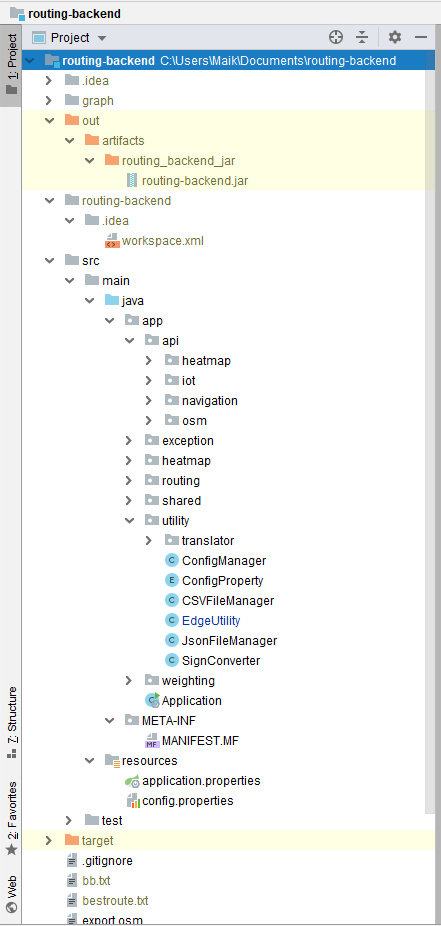
\includegraphics[width=8cm]{./ressourcen/routing/Ordnerstruktur-Routing.png}
	\caption{Ordnerstruktur der Routing-Komponente}
	\label{fig:folderstructure-routing}
\end{figure}

\Fig{folderstructure-routing} zeigt die Orderstruktur der Routing-Komponente.
Hier ist zu sehen, dass das Projekt aus zwei Hauptordnern besteht.
Diese sind der \textit{Java} und der \textit{resources} Ordner.

In dem \textit{resources} Ordner befinden sich zwei Config Dateien, in denen unter anderem der Server-Port oder die anzusprechenden Endpunkte angegeben werden.

In dem \textit{Java} Ordner befinden sich die Metadaten (\textit{MEAT-INF}) für die JAR-Datei und der Quellcode der Anwendung (\textit{app}).
Der \textit{app} Ordner ist unterteilt in die verschiedenen Teilkomponenten des Routing-Backends.
Hierzu zählen die Schnittstellen (\textit{api}), der Heatmap-Service (\textit{heatmap}), der Routing-Service (\textit{routing}), die Gewichtungs-Komponente (\textit{weighting}), ein Ordner für die allgemeine Funktionalitäten die an verschiedenen Stellen benötigt werden ({\textit{utility}) und ein Ordner in dem sich alle Klassen befinden die als Datenobjekte genutzt werden (\textit{shared}).

In dem \textit{api} Ordner gibt es Schnittstellen zur IoT-Plattform (\textit{heatmap}).
Hierüber werden die benötigten Daten zur Berechnung einer Route bzw. einer Heatmap abgefragt.
Außerdem gibt es noch Endpunkte die für die verschiedenen Frontends bereitgestellt werden. Erstens gibt es Endpunkte für die Navigationsanwendung(\textit{navigation}) und zweitens Endpunkte für die Heatmap (\textit{heatmap}).

In den Ordnern \textit{heatmap} und \textit{routing} befinden sich jeweils die Klassen die für die Berechnung der Heatmap bzw. der Route zuständig sind.

Der \textit{utility} Ordner enthält verschiedene Klassen mit Funktionalitäten, die von allen anderen Komponenten im Routing-Backend genutzte werden können. 
Hierzu gehören zum Beispiel die Translator Klassen, welche den Input des Nutzers überprüfen und umwandeln. 

Im \textit{weighting} Ordner befinden sich alle Klassen die für die Gewichtung der Kanten während der Routen-Berechnung zuständig sind.

Der \textit{shared} Ordner enthält alle Klassen, die als Datenstruktur im Routing-Backend genutzt werden, wie z.B. eine Route oder eine Heatmap.

Abschließend gibt es noch den \textit{exception} Ordner. 
Hierin befindet sich die Customexception, die für Fehlerrückmeldung genutzt wird.

\subsection{Technologien}
In diesem Abschnitt werden die wichtigsten Technologien beschrieben, die für die Entwicklung des Routing-Backends genutzt wurden.

Als Programmiersprache wurde Java verwendet, da es dafür die meisten Frameworks für Routing Algorithmen hab und die Studenten am meisten Erfahrung mit Java hatten.

Für die Routen Berechnung wurde das Framework GraphHopper genutzt. Hierdurch wurde die Implementierung eines eigenen Routing Algorithmus unnötig, da GraphHopper bereits A-Stern, Bidirektionalen Dijakstra und Contraction Hirachy. GraphHopper wird detaillierter in Kapitel Grundlagen im Dokument 1 beschrieben.

Als Entwicklungsumgebung wurde IntelliJ IDEA verwendet. Hier hätte aber ebenso eine andere Entwicklungsumgebung verwendet werden. Mit Intellij hatte die Studenten die besten Erfahrungen gemacht.

Außerdem wurde Maven verwendet um die Dependencies des Projekts einfacher verwalten zu können.

\subsection{Steps to Code}
In diesem Abschnitt werden die Schritte beschrieben, die durchgeführt werden müssen, um den Quellcode zu erweitern.

\begin{enumerate}
	\item Installiere IntelliJ IDEA\footnote{\url{https://www.jetbrains.com/idea/download/\#section=windows}}.
	\item Lade das Projekt aus dem Repository\footnote{\url{https://git.swl.informatik.uni-oldenburg.de/projects/PGRIO/repos/routing-backend/browse}} herunter.
	 \item Starte die IntelliJ IDEA Entwicklungsumgebung und öffne das Projekt (Datei -> Öffnen -> Projekt auswählen)
\end{enumerate}
	 
Jetzt kann begonnen werden den Quellcode zu bearbeiten. 
Wurde neuer Quellcode implementiert und der Entwickler möchte die Anwendung lokal starten kann er dies tun indem er die Main-Methode der Klasse \textit{Application} im Ordner \textit{app} startet. Über Postman kann man das Routing-Backend dann explorativ testen.

\subsection{Steps to Deploy}
Soll eine neue Version des Routing-Backends auf dem Develop-System deployt werden, müssen folgende Schritte durchgeführt werden.

\begin{enumerate}
	\item Führe mit Maven die Operation \textit{package} aus. Im Ordner \textit{target} wird eine Jar-Datei erstellt, die in den weiteren Schritten genutzt wird.
	\item Logge dich via Putty\footnote{\url{https://www.putty.org/}} auf der Develop-VM\footnote{\url{pg-rio-routing-dvlp.informatik.uni-oldenburg.de}} ein.
	\item Starte WinSCP und melde dich hier ebenfalls auf der Develop-VM an.
	\item Stoppe die auf der VM laufende Anwendung.
	\item Kopiere die neue lokal erzeugte Jar-Datei mit WinSCP auf die VM und überschreibe somit die alte Jar-Datei.
	\item Starte anschließend die neue Jar-Datei auf der VM.
\end{enumerate}
\subsection{Code Konventionen}
Als Grundlage für die Code Konventionen wurde die offiziellen Konventionen von Oracle genommen, die sehr verbreitet sind.